% Options for packages loaded elsewhere
\PassOptionsToPackage{unicode}{hyperref}
\PassOptionsToPackage{hyphens}{url}
%
\documentclass[
]{article}
\usepackage{amsmath,amssymb}
\usepackage{lmodern}
\usepackage{iftex}
\ifPDFTeX
  \usepackage[T1]{fontenc}
  \usepackage[utf8]{inputenc}
  \usepackage{textcomp} % provide euro and other symbols
\else % if luatex or xetex
  \usepackage{unicode-math}
  \defaultfontfeatures{Scale=MatchLowercase}
  \defaultfontfeatures[\rmfamily]{Ligatures=TeX,Scale=1}
\fi
% Use upquote if available, for straight quotes in verbatim environments
\IfFileExists{upquote.sty}{\usepackage{upquote}}{}
\IfFileExists{microtype.sty}{% use microtype if available
  \usepackage[]{microtype}
  \UseMicrotypeSet[protrusion]{basicmath} % disable protrusion for tt fonts
}{}
\makeatletter
\@ifundefined{KOMAClassName}{% if non-KOMA class
  \IfFileExists{parskip.sty}{%
    \usepackage{parskip}
  }{% else
    \setlength{\parindent}{0pt}
    \setlength{\parskip}{6pt plus 2pt minus 1pt}}
}{% if KOMA class
  \KOMAoptions{parskip=half}}
\makeatother
\usepackage{xcolor}
\usepackage[margin=1in]{geometry}
\usepackage{color}
\usepackage{fancyvrb}
\newcommand{\VerbBar}{|}
\newcommand{\VERB}{\Verb[commandchars=\\\{\}]}
\DefineVerbatimEnvironment{Highlighting}{Verbatim}{commandchars=\\\{\}}
% Add ',fontsize=\small' for more characters per line
\usepackage{framed}
\definecolor{shadecolor}{RGB}{248,248,248}
\newenvironment{Shaded}{\begin{snugshade}}{\end{snugshade}}
\newcommand{\AlertTok}[1]{\textcolor[rgb]{0.94,0.16,0.16}{#1}}
\newcommand{\AnnotationTok}[1]{\textcolor[rgb]{0.56,0.35,0.01}{\textbf{\textit{#1}}}}
\newcommand{\AttributeTok}[1]{\textcolor[rgb]{0.77,0.63,0.00}{#1}}
\newcommand{\BaseNTok}[1]{\textcolor[rgb]{0.00,0.00,0.81}{#1}}
\newcommand{\BuiltInTok}[1]{#1}
\newcommand{\CharTok}[1]{\textcolor[rgb]{0.31,0.60,0.02}{#1}}
\newcommand{\CommentTok}[1]{\textcolor[rgb]{0.56,0.35,0.01}{\textit{#1}}}
\newcommand{\CommentVarTok}[1]{\textcolor[rgb]{0.56,0.35,0.01}{\textbf{\textit{#1}}}}
\newcommand{\ConstantTok}[1]{\textcolor[rgb]{0.00,0.00,0.00}{#1}}
\newcommand{\ControlFlowTok}[1]{\textcolor[rgb]{0.13,0.29,0.53}{\textbf{#1}}}
\newcommand{\DataTypeTok}[1]{\textcolor[rgb]{0.13,0.29,0.53}{#1}}
\newcommand{\DecValTok}[1]{\textcolor[rgb]{0.00,0.00,0.81}{#1}}
\newcommand{\DocumentationTok}[1]{\textcolor[rgb]{0.56,0.35,0.01}{\textbf{\textit{#1}}}}
\newcommand{\ErrorTok}[1]{\textcolor[rgb]{0.64,0.00,0.00}{\textbf{#1}}}
\newcommand{\ExtensionTok}[1]{#1}
\newcommand{\FloatTok}[1]{\textcolor[rgb]{0.00,0.00,0.81}{#1}}
\newcommand{\FunctionTok}[1]{\textcolor[rgb]{0.00,0.00,0.00}{#1}}
\newcommand{\ImportTok}[1]{#1}
\newcommand{\InformationTok}[1]{\textcolor[rgb]{0.56,0.35,0.01}{\textbf{\textit{#1}}}}
\newcommand{\KeywordTok}[1]{\textcolor[rgb]{0.13,0.29,0.53}{\textbf{#1}}}
\newcommand{\NormalTok}[1]{#1}
\newcommand{\OperatorTok}[1]{\textcolor[rgb]{0.81,0.36,0.00}{\textbf{#1}}}
\newcommand{\OtherTok}[1]{\textcolor[rgb]{0.56,0.35,0.01}{#1}}
\newcommand{\PreprocessorTok}[1]{\textcolor[rgb]{0.56,0.35,0.01}{\textit{#1}}}
\newcommand{\RegionMarkerTok}[1]{#1}
\newcommand{\SpecialCharTok}[1]{\textcolor[rgb]{0.00,0.00,0.00}{#1}}
\newcommand{\SpecialStringTok}[1]{\textcolor[rgb]{0.31,0.60,0.02}{#1}}
\newcommand{\StringTok}[1]{\textcolor[rgb]{0.31,0.60,0.02}{#1}}
\newcommand{\VariableTok}[1]{\textcolor[rgb]{0.00,0.00,0.00}{#1}}
\newcommand{\VerbatimStringTok}[1]{\textcolor[rgb]{0.31,0.60,0.02}{#1}}
\newcommand{\WarningTok}[1]{\textcolor[rgb]{0.56,0.35,0.01}{\textbf{\textit{#1}}}}
\usepackage{graphicx}
\makeatletter
\def\maxwidth{\ifdim\Gin@nat@width>\linewidth\linewidth\else\Gin@nat@width\fi}
\def\maxheight{\ifdim\Gin@nat@height>\textheight\textheight\else\Gin@nat@height\fi}
\makeatother
% Scale images if necessary, so that they will not overflow the page
% margins by default, and it is still possible to overwrite the defaults
% using explicit options in \includegraphics[width, height, ...]{}
\setkeys{Gin}{width=\maxwidth,height=\maxheight,keepaspectratio}
% Set default figure placement to htbp
\makeatletter
\def\fps@figure{htbp}
\makeatother
\setlength{\emergencystretch}{3em} % prevent overfull lines
\providecommand{\tightlist}{%
  \setlength{\itemsep}{0pt}\setlength{\parskip}{0pt}}
\setcounter{secnumdepth}{-\maxdimen} % remove section numbering
\ifLuaTeX
  \usepackage{selnolig}  % disable illegal ligatures
\fi
\IfFileExists{bookmark.sty}{\usepackage{bookmark}}{\usepackage{hyperref}}
\IfFileExists{xurl.sty}{\usepackage{xurl}}{} % add URL line breaks if available
\urlstyle{same} % disable monospaced font for URLs
\hypersetup{
  pdftitle={Real data: CAPE Positive},
  pdfauthor={Itziar Irigoien, Patricia Mas-Bermejo, Sergi Papiol, Neus Barrantes-Vidal,; Araceli Rosa, and Concepción Arenas},
  hidelinks,
  pdfcreator={LaTeX via pandoc}}

\title{Real data: CAPE Positive}
\usepackage{etoolbox}
\makeatletter
\providecommand{\subtitle}[1]{% add subtitle to \maketitle
  \apptocmd{\@title}{\par {\large #1 \par}}{}{}
}
\makeatother
\subtitle{In: A guide to test association between Polygenic Risk Scores
and psychological and psychiatric traits: practical examples}
\author{Itziar Irigoien, Patricia Mas-Bermejo, Sergi Papiol, Neus
Barrantes-Vidal, \and Araceli Rosa, and Concepción Arenas}
\date{}

\begin{document}
\maketitle

\hypertarget{working-flow-and-code}{%
\subsection{Working flow and code}\label{working-flow-and-code}}

In this real data set there are 106 PRS, and a \textbf{binary Trait}
(\(CAPE_{Positive}\)), with gender, age, and two Principal Components as
covariates.

\begin{itemize}
\tightlist
\item
  Data reading
\end{itemize}

\begin{Shaded}
\begin{Highlighting}[]
\NormalTok{dat }\OtherTok{\textless{}{-}} \FunctionTok{read.table}\NormalTok{(}\StringTok{"Real\_data\_Positive.csv"}\NormalTok{, }\AttributeTok{header=}\ConstantTok{TRUE}\NormalTok{, }\AttributeTok{sep=}\StringTok{"}\SpecialCharTok{\textbackslash{}t}\StringTok{"}\NormalTok{, }\AttributeTok{dec=}\StringTok{"."}\NormalTok{, }\AttributeTok{row.names=}\DecValTok{1}\NormalTok{)}
\FunctionTok{names}\NormalTok{(dat) }\CommentTok{\#}
\end{Highlighting}
\end{Shaded}

\begin{verbatim}
##   [1] "Sex"           "Age"           "CAPE_Positive" "PRS.1"        
##   [5] "PRS.2"         "PRS.3"         "PRS.4"         "PRS.5"        
##   [9] "PRS.6"         "PRS.7"         "PRS.8"         "PRS.9"        
##  [13] "PRS.10"        "PRS.11"        "PRS.12"        "PRS.13"       
##  [17] "PRS.14"        "PRS.15"        "PRS.16"        "PRS.17"       
##  [21] "PRS.18"        "PRS.19"        "PRS.20"        "PRS.21"       
##  [25] "PRS.22"        "PRS.23"        "PRS.24"        "PRS.25"       
##  [29] "PRS.26"        "PRS.27"        "PRS.28"        "PRS.29"       
##  [33] "PRS.30"        "PRS.31"        "PRS.32"        "PRS.33"       
##  [37] "PRS.34"        "PRS.35"        "PRS.36"        "PRS.37"       
##  [41] "PRS.38"        "PRS.39"        "PRS.40"        "PRS.41"       
##  [45] "PRS.42"        "PRS.43"        "PRS.44"        "PRS.45"       
##  [49] "PRS.46"        "PRS.47"        "PRS.48"        "PRS.49"       
##  [53] "PRS.50"        "PRS.51"        "PRS.52"        "PRS.53"       
##  [57] "PRS.54"        "PRS.55"        "PRS.56"        "PRS.57"       
##  [61] "PRS.58"        "PRS.59"        "PRS.60"        "PRS.61"       
##  [65] "PRS.62"        "PRS.63"        "PRS.64"        "PRS.65"       
##  [69] "PRS.66"        "PRS.67"        "PRS.68"        "PRS.69"       
##  [73] "PRS.70"        "PRS.71"        "PRS.72"        "PRS.73"       
##  [77] "PRS.74"        "PRS.75"        "PRS.76"        "PRS.77"       
##  [81] "PRS.78"        "PRS.79"        "PRS.80"        "PRS.81"       
##  [85] "PRS.82"        "PRS.83"        "PRS.84"        "PRS.85"       
##  [89] "PRS.86"        "PRS.87"        "PRS.88"        "PRS.89"       
##  [93] "PRS.90"        "PRS.91"        "PRS.92"        "PRS.93"       
##  [97] "PRS.94"        "PRS.95"        "PRS.96"        "PRS.97"       
## [101] "PRS.98"        "PRS.99"        "PRS.100"       "PRS.101"      
## [105] "PRS.102"       "PRS.103"       "PRS.104"       "PRS.105"      
## [109] "PRS.106"       "PC1"           "PC2"
\end{verbatim}

Check that all variables you are interested in are properly read and
that there are not other variables you do not need as it is the case.

\bigskip

\begin{itemize}
\tightlist
\item
  Do not forget to declare the categorical variables as factors
\end{itemize}

\begin{Shaded}
\begin{Highlighting}[]
\NormalTok{dat}\SpecialCharTok{$}\NormalTok{Sex }\OtherTok{\textless{}{-}} \FunctionTok{as.factor}\NormalTok{(dat}\SpecialCharTok{$}\NormalTok{Sex)}
\NormalTok{dat}\SpecialCharTok{$}\NormalTok{CAPE\_Positive }\OtherTok{\textless{}{-}} \FunctionTok{as.factor}\NormalTok{(dat}\SpecialCharTok{$}\NormalTok{CAPE\_Positive)}
\end{Highlighting}
\end{Shaded}

\hypertarget{what-full-model-should-be-considered}{%
\subsection{1. What full model should be
considered?}\label{what-full-model-should-be-considered}}

First, given a particular PRS (named PRS.i), consider all the possible
full models:

\begin{itemize}
\tightlist
\item
  FM\(_{WI}\) : log(p/1-p) versus PRS.i + Sex + Age + PC1 + PC2
\item
  FM\(_{Sex}\): log(p/1-p) versus PRS.i + Sex + PRS.i,Sex + Age + PC1 +
  PC2
\end{itemize}

\hypertarget{how-to-make-a-prs-ranking-to-find-the-important-ones}{%
\subsection{2. How to make a PRS ranking to find the important
ones?}\label{how-to-make-a-prs-ranking-to-find-the-important-ones}}

As is described in the paper, for each model, calculate the Tjur's
coefficients of discrimination. If Nagelkerke's \(R^2\) is prefered, set
statistic=``PseudoR2'' in function orderBin(), and calculate their sum
\(S\).

According to S, list the PRSs in decreasing order:

\begin{Shaded}
\begin{Highlighting}[]
\CommentTok{\# Order the PRSs}
\NormalTok{out }\OtherTok{\textless{}{-}} \FunctionTok{orderBin}\NormalTok{(dat, }\AttributeTok{yname=}\StringTok{"CAPE\_Positive"}\NormalTok{, }\AttributeTok{prsname =} \StringTok{"PRS."}\NormalTok{, }\AttributeTok{statistic =} \StringTok{"D"}\NormalTok{)}
\FunctionTok{head}\NormalTok{(out)}
\end{Highlighting}
\end{Shaded}

\begin{verbatim}
##            Model1     Model2        Sum
## PRS.15 0.03458250 0.06713832 0.10172083
## PRS.16 0.03662211 0.06247882 0.09910094
## PRS.14 0.02913388 0.06465976 0.09379364
## PRS.11 0.02658133 0.06369724 0.09027858
## PRS.12 0.02415016 0.06359970 0.08774985
## PRS.10 0.02603126 0.06110069 0.08713195
\end{verbatim}

\begin{Shaded}
\begin{Highlighting}[]
\NormalTok{mainfilename }\OtherTok{\textless{}{-}} \StringTok{"Real\_data\_CAPE\_Positive"}
\NormalTok{filename }\OtherTok{\textless{}{-}} \FunctionTok{paste0}\NormalTok{(mainfilename, }\StringTok{"\_Ordered\_PRS.csv"}\NormalTok{)}
\FunctionTok{write.csv2}\NormalTok{(out,}\AttributeTok{file=}\NormalTok{filename)}
\end{Highlighting}
\end{Shaded}

Plot the sum of discrimination coefficients \(D\). Lines: in blue the
median; in black the mean.

\begin{Shaded}
\begin{Highlighting}[]
\NormalTok{out }\OtherTok{\textless{}{-}} \FunctionTok{data.frame}\NormalTok{(out) }
\NormalTok{n }\OtherTok{\textless{}{-}} \FunctionTok{dim}\NormalTok{(out)[}\DecValTok{1}\NormalTok{]}
\NormalTok{select }\OtherTok{\textless{}{-}} \FunctionTok{grep}\NormalTok{(}\StringTok{"Model"}\NormalTok{, }\FunctionTok{names}\NormalTok{(out), }\AttributeTok{value=}\ConstantTok{FALSE}\NormalTok{)}
\NormalTok{out}\SpecialCharTok{$}\NormalTok{effect }\OtherTok{\textless{}{-}}\NormalTok{ out}\SpecialCharTok{$}\NormalTok{Sum}
\NormalTok{sds }\OtherTok{\textless{}{-}} \FunctionTok{apply}\NormalTok{(out[, select], }\DecValTok{1}\NormalTok{, sd)}
\NormalTok{out}\SpecialCharTok{$}\NormalTok{lower }\OtherTok{\textless{}{-}}\NormalTok{ out}\SpecialCharTok{$}\NormalTok{effect }\SpecialCharTok{{-}}\NormalTok{ sds}
\NormalTok{out}\SpecialCharTok{$}\NormalTok{upper }\OtherTok{\textless{}{-}}\NormalTok{ out}\SpecialCharTok{$}\NormalTok{effect }\SpecialCharTok{+}\NormalTok{ sds}
\NormalTok{out}\SpecialCharTok{$}\NormalTok{rank }\OtherTok{\textless{}{-}}\NormalTok{ n}\SpecialCharTok{:}\DecValTok{1}


\FunctionTok{ggplot}\NormalTok{(}\AttributeTok{data=}\NormalTok{out, }\FunctionTok{aes}\NormalTok{(}\AttributeTok{y=}\NormalTok{rank, }\AttributeTok{x=}\NormalTok{effect, }\AttributeTok{xmin=}\NormalTok{lower, }\AttributeTok{xmax=}\NormalTok{upper)) }\SpecialCharTok{+}
  \FunctionTok{geom\_point}\NormalTok{() }\SpecialCharTok{+}
  \FunctionTok{geom\_errorbarh}\NormalTok{(}\AttributeTok{height=}\NormalTok{.}\DecValTok{1}\NormalTok{) }\SpecialCharTok{+}
  \FunctionTok{scale\_y\_continuous}\NormalTok{(}\AttributeTok{name=}\ConstantTok{NULL}\NormalTok{, }\AttributeTok{breaks=}\NormalTok{ n}\SpecialCharTok{:}\DecValTok{1}\NormalTok{, }\AttributeTok{labels=}\FunctionTok{row.names}\NormalTok{(out), }\AttributeTok{position=}\StringTok{"right"}\NormalTok{) }\SpecialCharTok{+}
  \FunctionTok{labs}\NormalTok{(}\AttributeTok{title=}\StringTok{\textquotesingle{}\textquotesingle{}}\NormalTok{, }\AttributeTok{x=}\StringTok{\textquotesingle{}Sum of D\textquotesingle{}}\NormalTok{, }\AttributeTok{y =} \StringTok{\textquotesingle{}PRS\textquotesingle{}}\NormalTok{) }\SpecialCharTok{+}
  \FunctionTok{geom\_vline}\NormalTok{(}\AttributeTok{xintercept=}\FunctionTok{mean}\NormalTok{(out}\SpecialCharTok{$}\NormalTok{effect), }\AttributeTok{color=}\StringTok{\textquotesingle{}black\textquotesingle{}}\NormalTok{, }\AttributeTok{linetype=}\StringTok{\textquotesingle{}dashed\textquotesingle{}}\NormalTok{) }\SpecialCharTok{+}
  \FunctionTok{geom\_vline}\NormalTok{(}\AttributeTok{xintercept=}\FunctionTok{median}\NormalTok{(out}\SpecialCharTok{$}\NormalTok{effect), }\AttributeTok{color=}\StringTok{\textquotesingle{}blue\textquotesingle{}}\NormalTok{, }\AttributeTok{linetype=}\StringTok{\textquotesingle{}dashed\textquotesingle{}}\NormalTok{) }\SpecialCharTok{+}
  \FunctionTok{theme\_minimal}\NormalTok{()}
\end{Highlighting}
\end{Shaded}

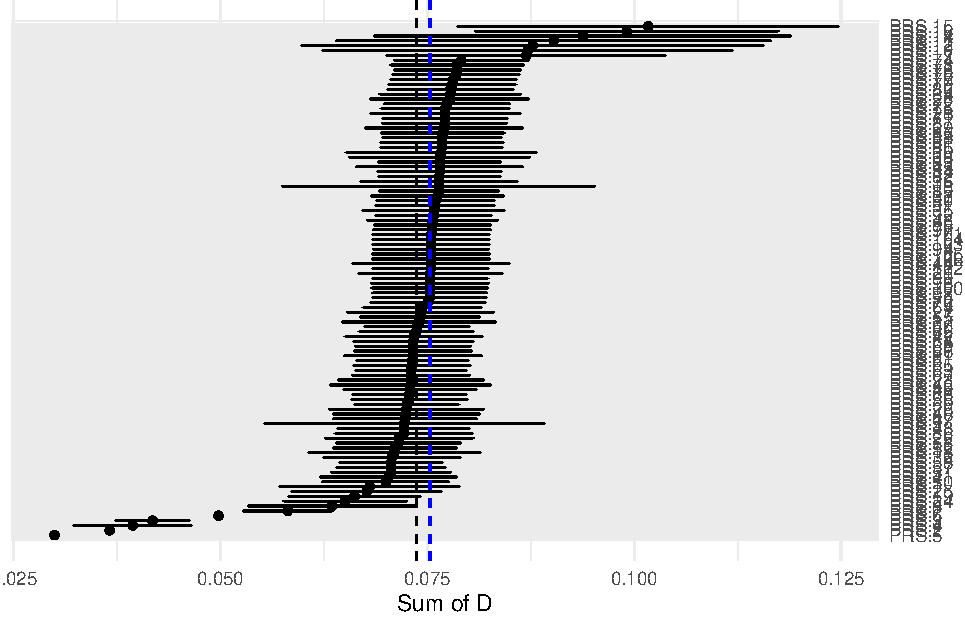
\includegraphics{Real_data_CAPE_Positive_code_files/figure-latex/unnamed-chunk-5-1.pdf}

According to the obtained results, first PRS.15 is selected to analyse
its association with the \(CAPE_{Positive}\).

\hypertarget{which-model-of-all-the-possible-ones-should-be-used}{%
\subsubsection{3. Which model, of all the possible ones, should be
used?}\label{which-model-of-all-the-possible-ones-should-be-used}}

The following Figure represents the scatter plot separated by Sex group.

\begin{Shaded}
\begin{Highlighting}[]
\CommentTok{\# First candidate PRS.15}
\CommentTok{\# Plot it}
\NormalTok{M }\OtherTok{\textless{}{-}} \FunctionTok{glm}\NormalTok{(CAPE\_Positive }\SpecialCharTok{\textasciitilde{}}\NormalTok{ PRS}\FloatTok{.15}\SpecialCharTok{*}\NormalTok{Sex }\SpecialCharTok{+}\NormalTok{ Age }\SpecialCharTok{+}\NormalTok{ PC1 }\SpecialCharTok{+}\NormalTok{ PC2, }\AttributeTok{data=}\NormalTok{dat, }\AttributeTok{family=}\FunctionTok{binomial}\NormalTok{())}
\NormalTok{pre }\OtherTok{\textless{}{-}}\NormalTok{ M}\SpecialCharTok{$}\NormalTok{fitted.values }\CommentTok{\#predict(M,type=\textquotesingle{}response\textquotesingle{})   }
\FunctionTok{xyplot}\NormalTok{(}\FunctionTok{log}\NormalTok{(pre}\SpecialCharTok{/}\NormalTok{(pre}\SpecialCharTok{+}\DecValTok{1}\NormalTok{))}\SpecialCharTok{\textasciitilde{}}\NormalTok{PRS}\FloatTok{.15}\SpecialCharTok{|}\NormalTok{Sex, }\AttributeTok{data=}\NormalTok{dat,  }\AttributeTok{type=}\FunctionTok{c}\NormalTok{(}\StringTok{"p"}\NormalTok{, }\StringTok{"r"}\NormalTok{))}
\end{Highlighting}
\end{Shaded}

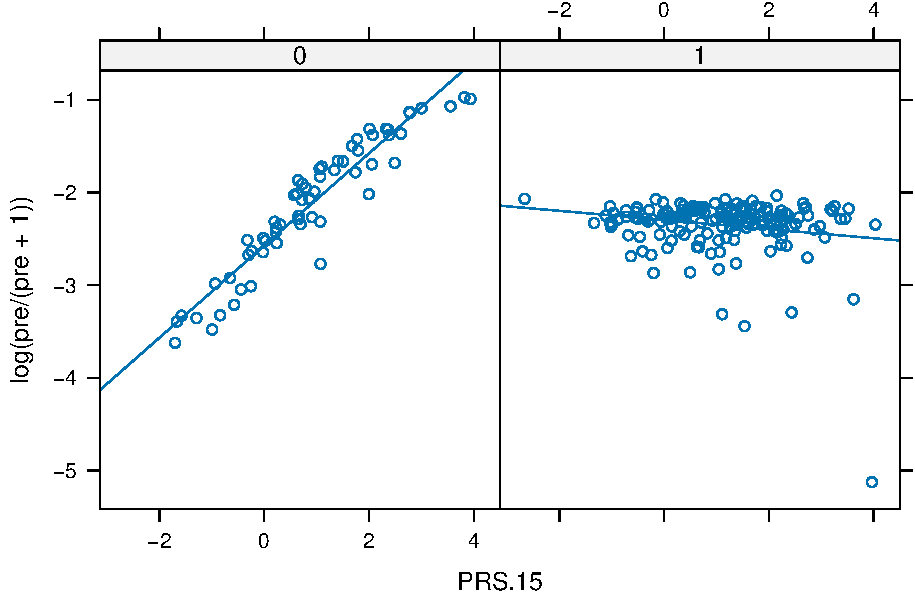
\includegraphics{Real_data_CAPE_Positive_code_files/figure-latex/unnamed-chunk-6-1.pdf}

The plots suggest that the interaction between the PRS.15 and the
diagnostic is relevant. Thus, we set the full model candidate (FM):
\(CAPE_{Positive} \sim PRS + Sex + PRS\cdot Sex + Age + PC1 +PC2\)

\hypertarget{for-a-binary-trait-what-steps-should-be-followed-for-a-correct-analysis}{%
\subsubsection{5. For a binary trait, what steps should be followed for
a correct
analysis?}\label{for-a-binary-trait-what-steps-should-be-followed-for-a-correct-analysis}}

Check for overdispersion

\begin{Shaded}
\begin{Highlighting}[]
\CommentTok{\#model}
\NormalTok{FM }\OtherTok{\textless{}{-}} \FunctionTok{glm}\NormalTok{(CAPE\_Positive }\SpecialCharTok{\textasciitilde{}}\NormalTok{ Sex }\SpecialCharTok{+}\NormalTok{ PRS}\FloatTok{.15}\SpecialCharTok{*}\NormalTok{Sex }\SpecialCharTok{+}\NormalTok{ Age }\SpecialCharTok{+}\NormalTok{ PC1 }\SpecialCharTok{+}\NormalTok{ PC2, }\AttributeTok{data=}\NormalTok{dat, }\AttributeTok{family=}\FunctionTok{binomial}\NormalTok{())}
\CommentTok{\#Residual Deviance}
\NormalTok{FM}\SpecialCharTok{$}\NormalTok{deviance}
\end{Highlighting}
\end{Shaded}

\begin{verbatim}
## [1] 165.7134
\end{verbatim}

\begin{Shaded}
\begin{Highlighting}[]
\CommentTok{\# Ratio }
\NormalTok{FM}\SpecialCharTok{$}\NormalTok{deviance}\SpecialCharTok{/}\NormalTok{FM}\SpecialCharTok{$}\NormalTok{df.residual}
\end{Highlighting}
\end{Shaded}

\begin{verbatim}
## [1] 0.7532427
\end{verbatim}

Since this ratio is close to 1, there is not evidence of overdispersion.

\begin{Shaded}
\begin{Highlighting}[]
\CommentTok{\#With chi{-}squared test}
\NormalTok{FM.od }\OtherTok{\textless{}{-}} \FunctionTok{glm}\NormalTok{(CAPE\_Positive }\SpecialCharTok{\textasciitilde{}}\NormalTok{ Sex }\SpecialCharTok{+}\NormalTok{ PRS}\FloatTok{.15}\SpecialCharTok{*}\NormalTok{Sex }\SpecialCharTok{+}\NormalTok{ Age }\SpecialCharTok{+}\NormalTok{ PC1 }\SpecialCharTok{+}\NormalTok{ PC2, }\AttributeTok{data=}\NormalTok{dat, }\AttributeTok{family=}\FunctionTok{quasibinomial}\NormalTok{())}
\FunctionTok{pchisq}\NormalTok{(}\FunctionTok{summary}\NormalTok{(FM.od)}\SpecialCharTok{$}\NormalTok{dispersion }\SpecialCharTok{*}\NormalTok{ FM}\SpecialCharTok{$}\NormalTok{df.residual,}
\NormalTok{       FM}\SpecialCharTok{$}\NormalTok{df.residual, }\AttributeTok{lower =}\NormalTok{ F)}
\end{Highlighting}
\end{Shaded}

\begin{verbatim}
## [1] 0.2651312
\end{verbatim}

With this p-value = 0.2651 we conclude that there is not evedence of
overdispersion.

Based on the estimations given in this table:

\begin{Shaded}
\begin{Highlighting}[]
\FunctionTok{summary}\NormalTok{(FM)}
\end{Highlighting}
\end{Shaded}

\begin{verbatim}
## 
## Call:
## glm(formula = CAPE_Positive ~ Sex + PRS.15 * Sex + Age + PC1 + 
##     PC2, family = binomial(), data = dat)
## 
## Coefficients:
##             Estimate Std. Error z value Pr(>|z|)  
## (Intercept)  0.05492    2.22416   0.025   0.9803  
## Sex1         0.13895    0.66711   0.208   0.8350  
## PRS.15       0.74628    0.28997   2.574   0.0101 *
## Age         -0.11833    0.10697  -1.106   0.2686  
## PC1          1.95129   14.54023   0.134   0.8932  
## PC2          2.86709   14.94056   0.192   0.8478  
## Sex1:PRS.15 -0.74871    0.35877  -2.087   0.0369 *
## ---
## Signif. codes:  0 '***' 0.001 '**' 0.01 '*' 0.05 '.' 0.1 ' ' 1
## 
## (Dispersion parameter for binomial family taken to be 1)
## 
##     Null deviance: 177.27  on 226  degrees of freedom
## Residual deviance: 165.71  on 220  degrees of freedom
## AIC: 179.71
## 
## Number of Fisher Scoring iterations: 5
\end{verbatim}

The PRS.15 coefficient will vary depending on the gender, being:

\begin{itemize}
\tightlist
\item
  \(\widehat{log(p/1-p)} = 0.055 + 0.746\times PRS.15 - 0.118\times Age + 1.951\times PC1 + 2.867\times PC2\),
  if Sex = 0.
\item
  \(\widehat{log(p/1-p)} = (0.055 + 0.139) + (0.746 - 0.749)\times PRS.15 - 0.118\times Age + 1.951\times PC1 + 2.867\times PC2\),
  if Sex = 1.
\end{itemize}

Check whether the respective PRS coefficients under each group are
significant or not.

\begin{Shaded}
\begin{Highlighting}[]
\FunctionTok{summary}\NormalTok{(}\FunctionTok{glht}\NormalTok{(FM, }\StringTok{"PRS.15 = 0"}\NormalTok{))}
\end{Highlighting}
\end{Shaded}

\begin{verbatim}
## 
##   Simultaneous Tests for General Linear Hypotheses
## 
## Fit: glm(formula = CAPE_Positive ~ Sex + PRS.15 * Sex + Age + PC1 + 
##     PC2, family = binomial(), data = dat)
## 
## Linear Hypotheses:
##             Estimate Std. Error z value Pr(>|z|)  
## PRS.15 == 0   0.7463     0.2900   2.574   0.0101 *
## ---
## Signif. codes:  0 '***' 0.001 '**' 0.01 '*' 0.05 '.' 0.1 ' ' 1
## (Adjusted p values reported -- single-step method)
\end{verbatim}

\begin{Shaded}
\begin{Highlighting}[]
\FunctionTok{summary}\NormalTok{(}\FunctionTok{glht}\NormalTok{(FM, }\StringTok{"PRS.15  + Sex1:PRS.15 = 0"}\NormalTok{))}
\end{Highlighting}
\end{Shaded}

\begin{verbatim}
## 
##   Simultaneous Tests for General Linear Hypotheses
## 
## Fit: glm(formula = CAPE_Positive ~ Sex + PRS.15 * Sex + Age + PC1 + 
##     PC2, family = binomial(), data = dat)
## 
## Linear Hypotheses:
##                            Estimate Std. Error z value Pr(>|z|)
## PRS.15 + Sex1:PRS.15 == 0 -0.002425   0.211998  -0.011    0.991
## (Adjusted p values reported -- single-step method)
\end{verbatim}

That means that for those with Sex=1, it seems that the PRS.15 is not
related to the Trait with odds = exp(-0.002) = 0.991, but for those with
Sex = 0 the model indicates that the coefficient of PRS.15 is 0.7463, so
the odds increase exp(0.7463) = 2.109 for an incremental of one unit in
PRS.15 with a p-value=0.0101.

It is possible to compute a permutation test to assess whether the
increase in the coefficient of determination \(D\) is significative.

\begin{Shaded}
\begin{Highlighting}[]
\CommentTok{\# Null model}
\NormalTok{NM }\OtherTok{\textless{}{-}} \FunctionTok{glm}\NormalTok{(CAPE\_Positive }\SpecialCharTok{\textasciitilde{}}\NormalTok{  Sex }\SpecialCharTok{+}\NormalTok{ Age }\SpecialCharTok{+}\NormalTok{ PC1 }\SpecialCharTok{+}\NormalTok{ PC2, }\AttributeTok{data=}\NormalTok{dat, }\AttributeTok{family=}\FunctionTok{binomial}\NormalTok{() )}
\NormalTok{permtest }\OtherTok{\textless{}{-}} \FunctionTok{dD}\NormalTok{(NM, FM, }\AttributeTok{seed=}\DecValTok{1236}\NormalTok{)}
\NormalTok{permtest}
\end{Highlighting}
\end{Shaded}

\begin{verbatim}
## $dD
##          1 
## 0.05246593 
## 
## $pvalue
## [1] 0.008
\end{verbatim}

In this particular case, it can be seen that the coefficient of
discrimination of the FM model is 0.05 units bigger than the
corresponding to the \emph{Null Model} NM, and it is statistically
significant.

\begin{itemize}
\tightlist
\item
  \textbf{Last step: We move to the next PRS.}
\end{itemize}

\end{document}
